%TCIDATA{LaTeXparent=0,0,relatorio.tex}
                      
\chapter{Resultados Experimentais}\label{CapExperimentos}

% Resumo opcional. Comentar se n�o usar.
%\resumodocapitulo{Resumo opcional.}

\section{Introdu��o}

A calibra��o 

\section{Dados de calibra��o dos transmissores de n�vel}

Pelo fato de a calibra��o dos transmissores de n�vel se dar de modo relativo, a aquisi��o dos dados e realiza��o do bloco de escala foi imediata, bastando tomar os dados do sensor com o tanque vazio e depois com o n�vel a 100\%. A Tabela~\ref{tab:dados_calib_nivel} mostra os dados tomados nessas circunst�ncias.

\begin{table}[h]
\centering
\caption{Dados para calibra��o dos transmissores de n�vel}
\label{tab:dados_calib_nivel}
\begin{tabular}{c|c|c|}
\cline{2-3}
 & \begin{tabular}[c]{@{}c@{}}\textbf{Dado do sensor [UD]}\\ (N�vel em 0\%)\end{tabular} & \begin{tabular}[c]{@{}c@{}}\textbf{Dado do sensor [UD]}\\ (N�vel em 100\%\end{tabular} \\ \hline
\multicolumn{1}{|c|}{\textbf{Sensor N�vel 1}} & 1072,1541                                                               & 22820,7862                                                                \\ \hline
\multicolumn{1}{|c|}{\textbf{Sensor N�vel 2}} & 879,7134                                                                & 22467,8037                                                                \\ \hline
\multicolumn{1}{|c|}{\textbf{Sensor N�vel 3}} & 886,7177                                                                & 22461,4197                                                                \\ \hline
\multicolumn{1}{|c|}{\textbf{Sensor N�vel 4}} & -73,0003                                                                & 21165,1354                                                                \\ \hline
\end{tabular}
\end{table}


	 
	 Como se v�, a simula��o do sinal de erro e de controle est� condizente com a aproxima��o do sistema em um modelo linear, acompanhando a sa�da real grande parte do tempo.

	 \begin{figure}[ht]
	 \center
	 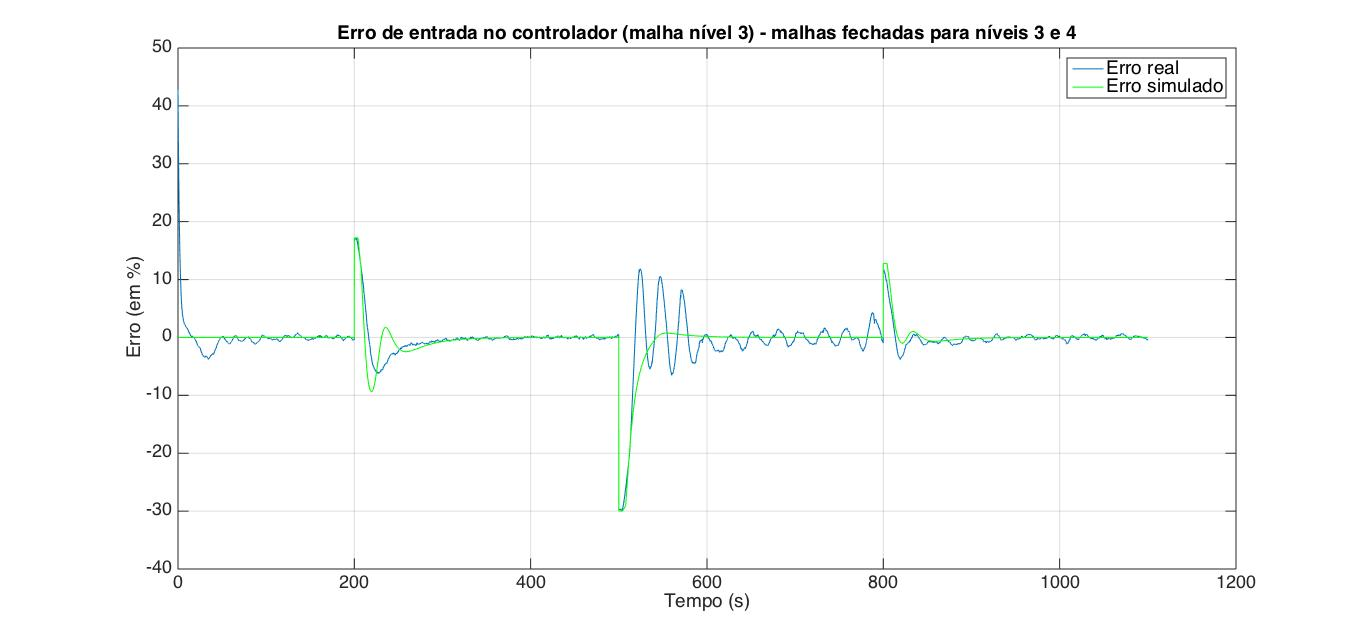
\includegraphics[scale=0.35]{figs/PI_H3H4_teste2_erro_H3.jpg}
	 \caption{Experimento 2: erro na entrada do PI-$B_2H_3$ - Controlador PI-$H_3H_4$ com novo valor inicial de bombas e anti-windup}
	 \label{f:PI_H3H4_teste2_erro_H3}
	 \end{figure}
	 
	
	 
	 \begin{figure}[ht]
	 \center
	 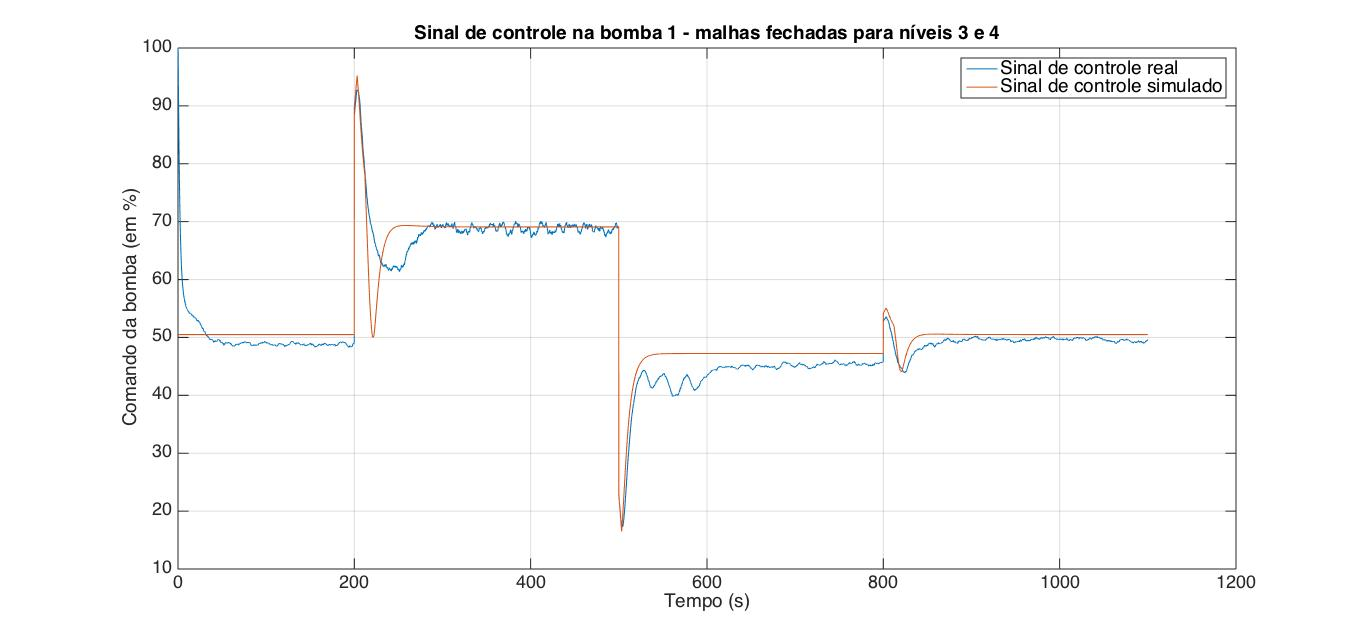
\includegraphics[scale=0.35]{figs/PI_H3H4_teste2_sig_B1.jpg}
	 \caption{Experimento 2: sinal de entrada na bomba 1 - Controlador PI-$H_3H_4$ com novo valor inicial de bombas e anti-windup}
	 \label{f:PI_H3H4_teste2_sig_B1}
	 \end{figure}
	 
